
\section{Introduction} % ================== 

Tobler's First Law of Geography says that things close together in space tend to behave more similarly than things further apart \citep{Tobler1970}. The model fit in Chapter 3 performs well, but we there of course remains unexplained spatial variation in the mean, and we assume missing covariate information. Accordingly, we augment the model with a spatially correlated random effect, giving a Spatial Generalized Linear Mixed Model (SGLMM). The spatial random effect can help account for some of the unexplained spatial variation in the mean, and help compensate for missing covariates \citep{Banerjee2008}. 

The random effect takes the form of a the Gaussian Random Field, which we introduce in the next section.

\subsection{Gaussian Random Field} % ================== 

A Gaussian random field (GRF) provides a tractable structure for spatial random effects in a linear model \citep{Gelfand2010}. To define a GRF, first define vector of locations $\pmb{s} \in \pmb{D} \subseteq \pmb{R}^{2}$, for spatial domain $\pmb{D}$. Then, define multivariate Normal random vector $\pmb{w}(\pmb{s})$, with mean $\pmb{0}$; and symmetric, positive definite covariance matrix $\Sigma(\pmb{\theta})$, with covariance parameters $\pmb{\theta}$ \citep{Haran2011}.
\begin{equation} \label{eq:w}
\pmb{w}(\pmb{s}) | \pmb{\theta} \sim MVN(\pmb{0}, \Sigma(\pmb{\theta})) 
\end{equation}
In sections \ref{stanopt} and \ref{ppm} we use a spatial exponential covariance structure for $\Sigma(\pmb{\theta})$. The i,jth element of the exponential covariance matrix, $\pmb{\Sigma}(\pmb{\theta})$, gives the covariance of the random effects $\pmb{w}(\pmb{s}_{i})$ and $\pmb{w}(\pmb{s}_{j})$:
\begin{equation} \label{eq:exp}
\Sigma(\phi, \sigma^{2})_{i,j} = \sigma^{2} exp(-||\pmb{s}_{i} - \pmb{s}_{j}||/\phi),
\end{equation}
with scale parameter $\sigma^{2}$, range parameter $\phi$, and where $||s_{i} - s_{j}||$ denotes the Euclidean distance between $\pmb{s}_{i}$ and $\pmb{s}_{j}$. In the next section we define the SGLMM we use.

\subsection{Spatial Generalized Linear Mixed Model}
Adding $\pmb{w}(\pmb{s})$ to the linear predictor in equation \ref{eq:glm} gives the following spatial generalized linear mixed model (SGLMM):
\begin{equation} \label{eq:SGLMM}
\text{logit}(p_{ij}|\pmb{s}_{ij}) = \pmb{X}_{ij}(\pmb{s}_{ij}) \pmb{\beta}_{j} + w(\pmb{s}_{ij}).
\end{equation}

This spatial model, containing a latent (unobserved) Gaussian random field, gives $\pmb{Y}$ a complicated correlation structure. Bayesian hierarchical spatial models most effectively accommodate this structure, and Markov chain Monte Carlo (MCMC) methods most effectively estimate model parameters \citep{Banerjee2014}. High dimensionality for this spatial model induces substantial computational costs, referred to as the ``Big N problem'' \citep{Lindgren2011}. We describe the Big N problem next.

\subsection{Three Approaches to the ``Big N Problem''}

Recall the multivariate Normal probability distribution function, for $\pmb{w}$ in our case.
\begin{equation} \label{eq:mvn}
f(\pmb{w}) = \frac{1}{(2\pi)^{n/2}|\Sigma|^{1/2}} \text{exp}\{ -\frac{1}{2}\pmb{w}'\Sigma^{-1}\pmb{w} \}
\end{equation}
Note that $|\Sigma|^{1/2}$ denotes the square root of the determinant of the n $\times$ n covariance matrix, and $\Sigma^{-1}$ denotes its inverse \citep{Lay}. For large sample sizes, these two components of the MVN distribution lead to prohibitive computational costs. To define the cost, we introduce ``big oh'' notation. 

For a sequence of two increasing functions $f(n)$ and $g(n)$, we say ``$f(n)$ is big `oh' $g(n)$ as n goes to infinity,'' or $f(n) = \mathcal{O}(g(n))$ as $n \rightarrow \infty$, if and only if there exists some $n_{0}$ and a positive real number M such that
  $$|f(n)| \leq \text{M} \cdot |g(n)| \text{ for all } n \geq n_0 $$
The computational costs of fitting a SGLMM with a latent GRF increase at a rate of $\mathcal{O}(n^{3})$ \citep{Finley2009}. We can define t(n) as time required to fit our model type to n observations; then:
$$t(n) \leq M \cdot n^{3} \text{ as } n \rightarrow \infty.$$
In less technical terms, this means the upper bound on the amount of time required for model fitting increases at the same rate as $n^{3}$. To understand why, refer back to the MVN pdf in equation \ref{eq:mvn}, and notice the n $\times$ n covariance matrix inverse and the determinant. Every MCMC algorithm iteration requires calculation and construction of these components; this accounts for the $\mathcal{O}(n^{3})$ rate of increase, prohibitively slow model fitting, and the ``Big N'' problem. 

To address these computational challenges, we tried three model-fitting approaches.
\begin{enumerate}
\item Computational optimization in Bayesian computing software Stan \citep{RSTAN}.
\item Dimension reduction with Predictive process models, implemented in R with the R package \verb|spBayes| \citep{Eidsvik2012}, \citep{Finley2013}.
\item Integrated Nested Laplace Approximations with Stochastic Partial Differential Equations, implemented in the R with the package \verb|INLA-R| \citep{Lindgren2015}.
\end{enumerate}
The first two approaches rely on the prevalent Bayesian model fitting algorithm  MCMC, the subject of the next section.

\subsection{Markov Chain Monte Carlo}

In Bayesian statistics we seek the posterior distribution of the parameter/s of interest, given the observed data. The fundamental Bayesian proportionality, for observation vector $\pmb{y}$, and parameter vector $\theta$, takes the form \citep{Gelman2014}:
\begin{equation} \label{eq:bayes}
p(\pmb{\theta}|\pmb{y}) \propto f(\pmb{y}|\pmb{\theta})p(\pmb{\theta}),
\end{equation}
with the posterior distribution of the parameters, given the data, proportional to the distribution of data given the parameters, times the prior distribution of the parameters. Elementary Bayesian models sometimes yield closed form posterior distributions, but more complex models rarely do. For complex models, MCMC offers an iterative procedure that converges to the true posterior distribution. This class of procedures presents its own challenges and weaknesses, but with sufficient computing power and time often provides the desired posterior distribution. The MCMC solution presents empirically, as draws from the posterior distribution of interest, rather than as a closed form. 

Markov chain properties supply the critical theoretical components of MCMC. Foremost among them, a sequence of possibly multivariate random variables $\pmb{X}_{1}, \pmb{X}_{2}, \hdots \pmb{X}_{n}$ possesses the Markov property if the distribution of $\pmb{X}_{n+1}|\pmb{X}_{1}, \pmb{X}_{2}, \hdots , \pmb{X}_{n}$ depends only on $\pmb{X}_{n}$. A sequence of random variables with the Markov property constitutes a Markov chain. MCMC algorithms use Markov chains that possess additional, necessary technical properties that assure an equilibrium distribution \citep{Brooks2011}. In fact, MCMC chains converge to an equilibrium distribution equivalent to the posterior distribution of interest.

Both Bayesian estimation programs used in this chapter use the Metropolis sampling algorithm, one of the most popular MCMC algorithms. \verb|Stan| uses HMC sampling and a ``Metropolis reject step'' \citep{STANtheMan}; while \verb|spBayes| uses a ``Metropolis-within-Gibbs'' sampler \citep{Finley2013}. 

In the next two sections we describe the Metropolis algorithm and the Gibbs sampler. The Metropolis algorithm manufactures draws from a distribution with a density function only known up to a proportionality constant; while the Gibbs sampler draws, often using the Metropolis, from a sequence of conditional distributions that converges to the posterior distribution of interest.

\subsubsection{Metropolis Algorithm } % \citep{Banerjee2014}

Often we don't have the closed form for a target distribution, such as an MCMC iteration conditional distribution, or the full posterior distribution. However, we always know the target distribution up to a proportionality constant, and thus have the posterior kernel. Let $h(\pmb{\theta})$ denote the posterior distribution kernel. The Metropolis algorithm uses $h(\pmb{\theta})$ to iteratively draw samples from the full conditionals, $p(\theta_{i}|\pmb{\theta}_{-i})$; and essentially reduce a high dimensional problem to a series of lower dimension problems. 

The algorithm requires a  candidate density, $q(\pmb{\theta}_{t}|\pmb{\theta}_{t-1})$, that we can readily draw samples from; whose support contains all possible values of $\pmb{\theta}_{t}$ and $\pmb{\theta}_{t-1}$; and is symmetric, ($q(\pmb{\theta}_{t}|\pmb{\theta}_{t-1}) = q(\pmb{\theta}_{t-1}|\pmb{\theta}_{t})$). Then, for $(t \in 1:T)$, with T prescribed iterations, we choose an initial value $\pmb{\theta}_{0}$ for $\pmb{\theta}$, and the algorithm proceeds as follows.
\begin{enumerate}
\item Generate candidate value of $\pmb{\theta}$, call it $\pmb{\theta}^{*}$, from $q(\pmb{\theta}^{*}|\pmb{\theta}_{t})$.
\item Compute the ratio of kernels,
$$ r=h(\pmb{\theta}^{*})/h(\pmb{\theta}^{t-1}) = \text{exp}[\text{log }h(\pmb{\theta}^{*}) - \text{log }h(\pmb{\theta}^{(t-1)}). $$
\item If $r \geq  1$, set $\pmb{\theta}^{t} = \pmb{\theta}^{*}$; \\
            If $r < 1$, set 
            \[ 
            \pmb{\theta}^{t} = 
            \begin{cases} 
            \pmb{\theta}^{*} \text{ with probability r} \\
            \pmb{\theta}^{(0)} \text{ with probability 1 - r} \\
            \end{cases}
            \]
  \end{enumerate}
This algorithm successfully draws samples from a distribution known only up to a proportionality constant.   

\subsubsection{Gibbs Sampler}
In high dimensional problems that are now common, the Gibbs Sampler achieves success, in part, because it iteratively reduces the dimension of the problem. To understand how, and delineate the algorithm, first define parameter vector $\pmb{\theta} = (\theta_{1}, \dots, \theta_{k})'$. We assume here we can draw samples from $p(\theta_{i}|\theta_{j \neq i},y)$ directly, or use the Metropolis algorithm described in the previous section. The Gibbs sampler proceeds with the following steps, for iterations $(t \in 1:T)$ \citep{Banerjee2014}. 
        \begin{itemize} 
        \item Step 1: draw $\theta_{1}^{t}$ from $p \left( \theta_{1}|\theta_{2}^{t-1}, \theta_{3}^{t-1},\dots,\theta_{k}^{t-1},\pmb{y} \right)$ 
        \item Step 2: draw $\theta_{2}^{t}$ from $p \left(\theta_{2}|\theta_{1}^{t}, \theta_{3}^{t-1},\dots,\theta_{k}^{t-1},\pmb{y} \right)$ \\
        $\vdots$
        \item Step k: draw $\theta_{k}^{t}$ from $p \left( \theta_{k}|\theta_{1}^{t}, \theta_{3}^{t},\dots,\theta_{k-1}^{t},\pmb{y} \right)$ 
        \item Repeat for all $(t \in 1:T)$
        \end{itemize} 
If the chain satisfies certain regularity conditions, as it does in MCMC usage, then the iterations converge to draws from the true posterior distribution $p(\pmb{\theta}|\pmb{y})$ \citep{Banerjee2014}. 


In the next section we present our first attempt to address the big N computational problem: optimization techniques in Stan. As mentioned, Stan uses the Metropolis algorithm with an unusual proposal mechanism.

\section{Optimization in Stan} \label{stanopt} % =================

The Metropolis algorithm requires a proposal distribution or some other kind of  generating mechanism. Often a random walk distribution, or some other accessible distribution, plays this role. On the other hand, Stan uses a proposal mechanism that originated in physics, Hamiltonian Monte Carlo (HMC), to generate proposals for the Metropolis reject step. HMC generates well mixed, high probability proposals---both important factors. Mixing refers to the degree to which proposals explore the parameter support, and acceptance rates refer to the likelihood that the algorithm accepts proposals as draws from the target distriubtion. Insufficient mixing and low acceptance rates delay, or even prevent, the sampling algorithm from converging to its equilibrium distribution. An acceptance rate too high signals insufficient mixing and potentially overly correlated draws. In Stan's MCMC, HMC balances the proposal mechanism demands well. 

This fascinating HMC method originates in physics, which we describe in the next section.

\subsection{Hamiltonian Monte Carlo} 

Trying to understand molecular states, \cite{Metropolis1953} created MCMC for ``fast machines.'' Later, modeling molecular motion as a deterministic process, \cite{Alder1959} introduced {\it Hamiltonian dynamics} as an alternate representation of Newtonian mechanics. Almost 30 years later, \cite{Duane1987} combined the two to create ``hybrid Monte Carlo,'' using it to simulate quantum mechanical processes. Over time, the name morphed into {\it Hamilton} Monte Carlo (HMC). Eventually HMC made its way into statistics, when \cite{Neal1996} used HMC to study neural networks.

HMC works by reframing the variables and distribution of interest as position variables in a physical system, and artificially introducing momentum variables to perturb the position. To better understand, imagine a puck with known position and momentum on a frictionless surface, and then randomly changing the momentum of the puck to alter its course. HMC treats the variables of interest as position variables, and uses randomly generated auxiliary Gaussian variables to change the momenturm. Then, the new position, calculated with a set of differential equations, provides proposals for Metropolis updates. The differential equation solutions estimate trajectories of the hypothetical physical object (the puck), which then occupies a new position after a time step of some chosen duration. This crafty formulation provides distant (well mixed), yet high probability (high acceptance rate) proposals. This contrasts favorably with the random walk proposal generation process commonly used.\footnote{I dedicate this section to my high school physics teacher, the late William T. Meyers. He helped instill in me a love of physics, and emphasized that in his class we would learn critical thinking skills that we could use in our life.}

\subsection{The Hamilton Equations} % =================

To define the Hamilton equations for d variables of interest, let d-dimensional position vector $q(t)$ depend on time $t$; and let $U(q(t))$ denote the potential energy at time $t$. Let $p(t)$ give the d-dimensional momentum at time $t$, and $K(p(t))$ denote kinetic energy at time $t$. Then the Hamilton equation,
\begin{equation}
H(q(t),p(t)) = U(q(t)) + K(p(t)),
\end{equation}
measures the total energy of a system as a function of potential and kinetic energy. 

In HMC applications, we let the potential energy, $U(q)$, be minus the log of the probability density function of interest, plus a constant.\footnote{We omit $t$ for clarity of presentation, here and elsewhere, but position and momentum remain functions of time $t$.} Next, define d-dimensional vector $p$ as a zero mean Gaussian random variable with covariance matrix M, and define $K(p)$ as minus the log of the multivariate Gaussian probability density function. This gives the Hamilton equation form:
\begin{equation} \label{eq:ham}
H(q,p) = -\text{log}f_{q}(q) + p^{T}\pmb{M}^{-1}p/2.
\end{equation}
This formulation yield tractable partial derivatives for calculating the change in position and momentum through time. For $i = 1,\dots, \text{d}$:
\begin{align}
\frac{d q_{i}(t)}{dt} &= \frac{\partial H}{\partial p_{i}}, \\
\frac{d p_{i}(t)}{dt} &= -\frac{\partial H}{\partial q_{i}}.
\end{align}
Substituting equation \ref{eq:ham} and simplifying gives:
\begin{align}
\frac{d q_{i}(t)}{dt} &=  [\pmb{M}^{-1}p]_{i} \\
\frac{d p_{i}(t)}{dt} &= \frac {\partial \left[ \text{log}f_{q}(q) \right]}{\partial q_{i}}
\end{align}
The differential equation solutions give the position and momentum at time t. With solutions in hand, the ``leapfrog method'' calculates changes in the Hamilton through small time steps, by discretizing the continuously defined Hamilton equation using Taylor Series approximations \citep{Neal2011}. 

In summary, the HMC algorithm samples from the auxiliary Normal distribution, and then calculates the proposal as the positions vector in the Hamilton equation. This method yields high probability, well mixed Metropolis proposals. This combination, and Stan's reputation for efficient Bayesian model fitting, motivated us to use Stan for model fitting. The next section describes techniques specific to Stan, for fast, efficient model fitting. 

\subsection{Optimization Techniques} % =================
With the techniques presented in this section, we aimed to improve Stan model fitting efficiency enough to successfully fit our SGLMM to thousands, or tens of thousands, of observations. The techiques include Bayesian, linear algebra, and purely computational strategies. We start with techniques related to the Bayesian model components.

Stan permits users to omit prior distributions for parameters, but then assumes a non-informative, uniform prior for that parameter. However, Andrew Gelman pointed out in personal correspondence that the exponential covariance range parameter, $\phi$ in equation \ref{eq:exp}, requires an informative prior for model identifiability (uniqueness) \citep{Gelman2014}. In this vein, Stan developer Rob Trangucci recommended, also in personal correspondence, a sharp tailed prior distribution for range parameter $\phi$, such as the normal or log-normal, to act as soft upper and lower bound constraints \citep{Trangucci}. Even further, for practical computing time and convergence considerations, Trangucci indicated complex models---such as spatial hierarchical models---require proper priors for all $\beta$ coefficients \citep{Trangucci}. The next two techniques combine linear algebra and computational considerations.

For all operations in Stan, matrix algebra and vectors acheive greater speed and efficiency than loops and scalars \citep{STANtheMan}. For example, 
\begin{verbatim}
hit ~ bernoulli_logit(X*beta + Z)
\end{verbatim}
runs faster than
\begin{verbatim}
for (n in 1:N)
        hit[n] = bernoulli_logit(X[n]*beta[n] + Z[n])
\end{verbatim}
The first, faster line includes N$\times$1 column vectors \verb|hit|, \verb|beta|, and \verb|Z|; and N$\times$p matrix \verb|X|. The second, slower snippet, instead uses scalars \verb|hit[n]|, \verb|beta[n]|, and \verb|Z[n]|; and 1$\times$p row vector \verb|X[n]|.

Trangucci also suggested a QR factorization on covariate matrix $\pmb{X}$, in the linear predictor, to increase computational efficiency \citep{Trangucci}. A QR factorization consists of factoring an n $\times$ p matrix into the product of an n $\times$ p orthogonal matrix $\pmb{Q}$ and a p $\times$ p upper triangular matrix $\pmb{R}$, such that $\pmb{X} = \pmb{QR}$. Leveraging this factorization into a speed increase requires a reparameterization. To this end, let $\pmb{\theta} = \pmb{R \beta}$, which gives:
\begin{align}
\pmb{X} &= \pmb{QR} \\
\pmb{X \beta} &= \pmb{QR \beta} \\
\pmb{X \beta} &= \pmb{Q \theta},
\end{align}
and the model
\begin{equation} \label{eq:reparam}
\text{logit}(p_{ij}|\pmb{s}_{ij}) = \pmb{Q}_{ij}(\pmb{s}_{ij}) \pmb{\theta}_{j} + w_{ij}.
\end{equation}
With this parameterization we incorporate prior information about $\pmb{\beta}$ in the $\pmb{\theta}$ prior distributions. 

Consider non-informative prior distributions on p-dimensional parameter vector $\pmb{\beta}$,
\begin{equation}
\pmb{\beta} \sim N(\pmb{0}, \sigma^{2}\pmb{I}_{p}), 
\end{equation}
with p $\times$ p identity matrix $\pmb{I}_{p}$; and p $\times$ 1 zero vector $\pmb{0}$. Notice the intended variance of the non-informative prior must be modified, to be on the scale of $\pmb{\theta}$.
\begin{align}
\text{Var}(\pmb{\theta}) &= \text{Var}(\pmb{R \beta}) \\
&= \pmb{R}\text{Var}(\pmb{\beta})\pmb{R}' \\
&= \pmb{R}\sigma^{2}\pmb{I}_{p}\pmb{R}' \\
&= \sigma^{2} \pmb{R}\pmb{R}'
\end{align}
This essential follow-up adjustment ensures appropriate weighting of prior information. Next, we look at a purely computational modification.

While we chose a covariance structure meeting all necessary criteria, we add computational noise to the covariance matrix diagonal, with the following snippet of code, to ensure {\it numerical} positive-definiteness.
\begin{verbatim}
for (n in 1:N)
  Sigma[n, n] = Sigma[n, n] + 1e-6;
\end{verbatim}
The stan function \verb|cov_exp_quad(...)| assembles the covariance matrix, and the added diagonal noise guarantees that it remains numerically positive-definite \cite{Trangucci2017}. This reduces wasted MCMC iterations, because \verb|cov_exp_quad(...)| can generate numerically non-positive-definite matrices when operating at high dimensions.

Finally, Stan developer Bob Carpenter recommended, in personal communication, a Cholesky decomposition and reparameterization, noting the efficiency of a vectorized scalar approach \cite{Carpenter}.
\begin{verbatim}
L = cholesky_decompose(Sigma);  
Z ~ normal(0, 1);  
Z_mod = L * Z; 
hit ~ bernoulli_logit(Q*theta + Z_mod);
\end{verbatim}
The first line performs a Cholesky decomposition on the covariance matrix \verb|Sigma|, by finding lower triangular matrix \pmb{L} such that $\Sigma = \text{\pmb{LL}}'$. Line 2, ``vectorized scalar'' \verb|Z ~ normal(0, 1)| generates n standard normal random variables, by reusing ``\verb|normal(0, 1)|'' for every element of \verb|Z|. These two lines remove the dependence of random vector \pmb{Z}, which must be generated, on the unknown parameters \citep{Trangucci2017}. The third line, \verb|Z_mod = L * Z|, uses \verb|L| to transform \verb|Z|, so that \verb|Z_mod| possesses the desired distribution. Note that $\text{Var}(\text{\pmb{LZ}}) = \text{\pmb{L}} \text{I}_{n}\text{\pmb{L}}' = \Sigma$, so that $\pmb{LZ} \sim N(\pmb{0}, \Sigma)$ as desired. The final line specifies the model.

This collection of techniques improved the model fit efficiency somewhat, which we discuss in the next section.

\subsection{Results}

In initial model fitting, using a test data set of n = 25 observations, to sample one 500 sample chain required approximately 50 seconds of computing time. Using the Cholesky decomposition described above reduced this time to 26 seconds. Proper priors on covariance parameters and noise on the covariance diagonal drastically reduced the number of numerical/sampling errors and warning messages, shaving another few seconds off the computing time. Using proper, non-informative priors for all elements of $\pmb{\beta}$ reduced computing time for n=25 observations to approximately 5 seconds. 

However, increasing the number of observations to n=500 required approximately 100 minutes; increasing the observations by a factor of 20 increased the computing time by a factor of 1200. The $\pmb{QR}$ decomposition yielded significant further gains: n = 1000 observations required about 60 minutes. As a point of reference, fitting a GLM---without a spatial random effect---with the same number of observations required about six {\it seconds}. Despite these improvements, Stan-based modeling efforts ended at n = 2000, when an overnight MCMC fit attempt yielded only 350 of 500 samples.

Optimization in Stan proved inadequate for addressing the ``big N'' problem. Next, in an effort to address the big N problem in another way, we examine an approach that creates a reduced dimension representation of a SGLMM. 

\section{Dimension Reduction with Predictive Process Models} \label{ppm} % ======

\subsection{Introduction}

Predictive process models (PPMs) reduce the dimension of our SGLMM's covariance matrix to circumvent the big N problem. Several general strategies exist for this task, with often several methods to implement each strategy. \cite{Fuentes2007} and \cite{Paciorek2007} use a spectral representation of the covariance function, and Fourier transforms, to reduce the dimensionality of data on a regular lattice. ``Covariance tapering'' involves setting small values in the covariance matrix to zero, and achieving computational gains that come with a sparse matrix \citep{Furrer2006}, \citep{Kaufman2008}. We explore one computational approximation approach in Section \ref{INLA} \citep{Rue2009}, but others exist \citep{Stein2004}, \citep{Eidsvik2014}, \citep{Aune2014}. Still more apply exact methods to a simplified, lower rank version of the original model \citep{Cressie2008}, \citep{Higdon2002}, \citep{Eidsvik2012}. The next strategy we use, PPMs, belongs to this latter category.

PPMs provide a competitive modeling approach, but one with computational advantages specific to hierarchical models with a GRF at the second level of specification---such as our SGLMM \citep{Banerjee2008}. Gaussian PPMs project the original spatial process onto a lower dimensioned subspace, at a set of locations called knots, to achieve dimension reduction \citep{Banerjee2008}. In the next section we describe this procedure in detail, defining additional notation as necessary.

\subsection{PPM Procedure}
Consider again the SGLMM from equation \ref{eq:SGLMM}, defined as it was there, and Gaussian random field $\pmb{w}(\pmb{s})$.
\begin{align}
\text{logit}(p_{ij}|\pmb{s}_{ij}) &= \pmb{X}_{ij}(s_{ij}) \pmb{\beta}_{j} + w(\pmb{s}_{ij}) \label{eq:ppm} \\
\pmb{w}(\pmb{s}) | \pmb{\theta} &\sim \text{GRF}(\pmb{0}, \pmb{C}(\pmb{\theta})) \label{eq:GRF}
\end{align}
Equation \ref{eq:GRF} defines a stationary GRF for n $\times$ 1 vector of random effects $\pmb{w}$, at locations $\pmb{s}$, conditioned on covariance parameters $\pmb{\theta}$; with mean  n $\times$ 1 zero vector $\pmb{0}$; and a symmetric, positive-definite, n $\times$ n covariance matrix $\pmb{C}(\pmb{\theta})$.

To begin to define the PPM procedure, let $C(\pmb{s}_{i}, \pmb{s}_{j}; \pmb{\theta})$ denote the covariance of random effects at locations $\pmb{s}_{i}$ and $\pmb{s}_{j}$, so that $C(\pmb{\theta}) = [C(\pmb{s}_{i}, \pmb{s}_{j}; \pmb{\theta})]_{i,j=1}^{n}$. Next, let $\pmb{S}^{*} = \{\pmb{s}_{1}^{*}, \dots, \pmb{s}_{m}^{*}\}$ give a set of $m << n$ chosen knot locations, not necessarily a subset of observed locations. \footnote{Knot selection, a non-trivial decision, is equal to the area of study known as spatial sampling design \citep{Finley2009}. See \citep{Xia2006} for a summary of spatial sampling approaches.} We denote knot location random effects with m $\times$ 1 vector $\pmb{w}^{*} = \left[w(\pmb{s}_{i}^{*})\right]_{i=1}^{m}$, and the m $\times$ m knot covariance matrix and its elements as $\pmb{C}^{*}(\pmb{\theta}) = \left[C(\pmb{s}_{i}^{*}, \pmb{s}_{j}^{*})\right]_{i,j = 1}^{m}$. The knot random effects constitute a distinct m-dimensional GRF:
\begin{equation}
\pmb{w}^{*}|\pmb{\theta} \sim \text{GRF}\{\pmb{0}, \pmb{C}^{*}(\pmb{\theta})\}.
\end{equation}

Consider a new loction $\pmb{s}_{0}$. The PPM procedure uses the m knots, the covariance structure of the parent process, and kriging to interpolate $w$ at $\pmb{s}_{0}$ \citep{Schabenberger2004}. To see this, let $\tilde{w}(\pmb{s}_{0})$ represent this interpolated random effect, and let $\pmb{c}(\pmb{s}_{0};\pmb{\theta}) = \left[C(\pmb{s}_{0}, \pmb{s}_{j}^{*}; \pmb{\theta})\right]_{j = 1}^{m}$ be an m $\times$ 1 covariance vector giving the covariance of the $\pmb{s}_{0}$ random effect with the knot random effects. Then,  kriging estimator
\begin{align}
\tilde{w}(\pmb{s}_{0}) &= E[w(\pmb{s}_{0})|\pmb{w}^{*}] \\ 
&= \pmb{c}^{T}(\pmb{s}_{0};\pmb{\theta}) \cdot \pmb{C}^{*-1}(\pmb{\theta}) \cdot \pmb{w}^{*} \label{eq:krig}
\end{align}
minimizes the squared error loss function among all linear predictors \citep{Schabenberger2004}. Notice that the linear combination (\ref{eq:krig}) varies spatially. Accordingly, predictive process $\tilde{w}(\pmb{s})$ defines the following GRF and covariance matrix.
\begin{align}
\tilde{\pmb{w}}(\pmb{s}) &\sim \text{GRF}\{0, \tilde{C}(\cdot)\} \\
\tilde{C}(\pmb{s}, \pmb{s}'; \pmb{\theta}) &= \pmb{c}^{T}(\pmb{s};\pmb{\theta}) \cdot \pmb{C}^{*-1}(\pmb{\theta}) \cdot \pmb{c}(\pmb{s}';\pmb{\theta})
\end{align}
Recall m $\times$ 1 vector $\pmb{c}(\pmb{s};\pmb{\theta}) = \left[C(\pmb{s}, \pmb{s}_{j}^{*})\right]_{j = 1}^{m}$ gives the covariance of the random effect at $\pmb{s}$ with knot random effects. This last GRF replaces the full GRF in the parent process, to give the following PPM.
\begin{equation}
\text{logit}(p_{ij}|\pmb{s}_{ij}) = \pmb{X}_{ij}(\pmb{s}_{ij}) \pmb{\beta}_{j} + \tilde{w}(\pmb{s})
\end{equation}
We used the R package  to implement the PPM approach to dimension reduction. We present the results in the next section.

\subsection{Results and Discussion}

R package \verb|spBayes| provides function \verb|spGLM(...)|, which we used to fit our SGLMM \citep{Finley2013}. Using PPMs requires  knot selection, and the number of knots, some $m < < n$, directly imacts the computational costs. Using a range of values for $m$, PPMs drastically outperformed Stan optimization big N model fitting. 

In our model fits with PPMs, we used VR heat map box centers for knots. In our first set of model fits, we used 97 VR heat map box centers as knots. 
  \begin{figure}[H]
	\centering 
	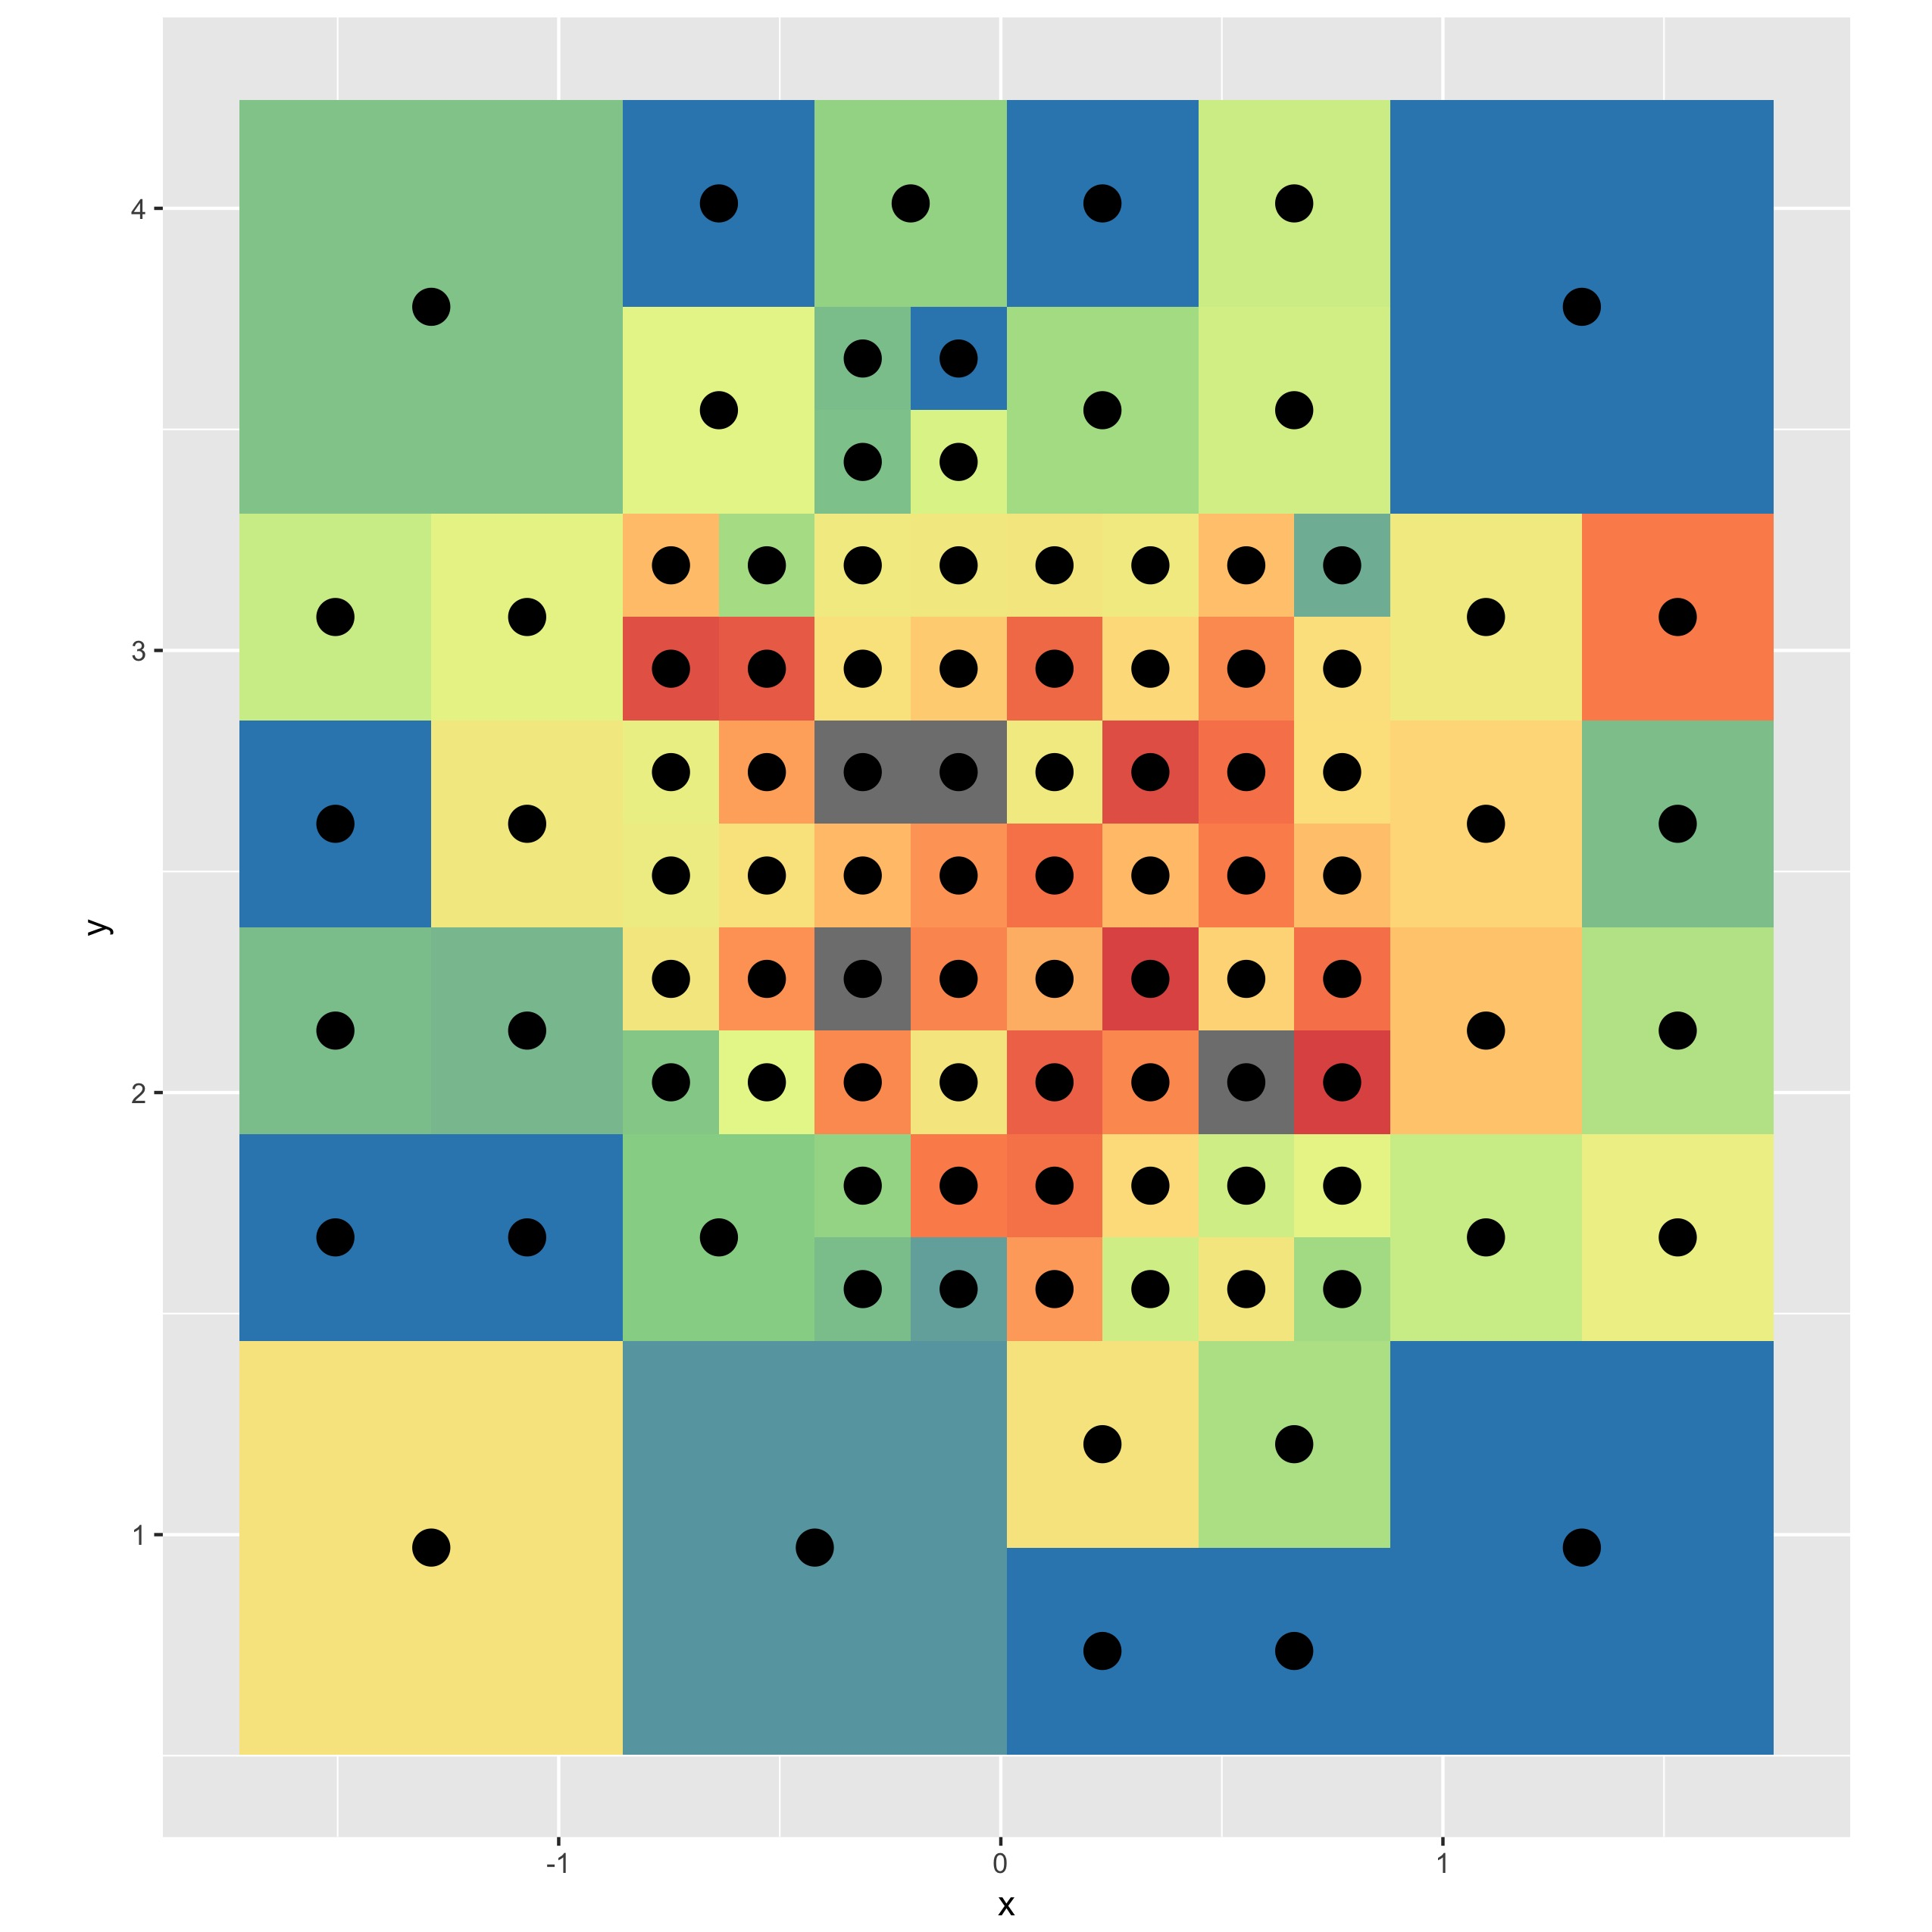
\includegraphics[scale=.1]{Images/knots.jpg}
	\caption{This map shows 97 PPM knots as variable-resolution heat map box centers. This Jhonny Peralta map used stopping rule $n_{b} < 200$.}
	\end{figure}


Using these 97 knots, for n = 300 observations, the PPM model fit generated 10,000 samples in three minutes. For n = 500 observation, 10,000 posterior draws required 4 minutes. For the same number of knots, but n = 1000 observations, 10,000 posterior draws required less than seven minutes; and 37,500 draws required 23 minutes. The follow graphic shows VR empirical, GLM, and PPM fits for the same random n = 1000 subsample.

  \begin{figure}[H]
	\centering 
	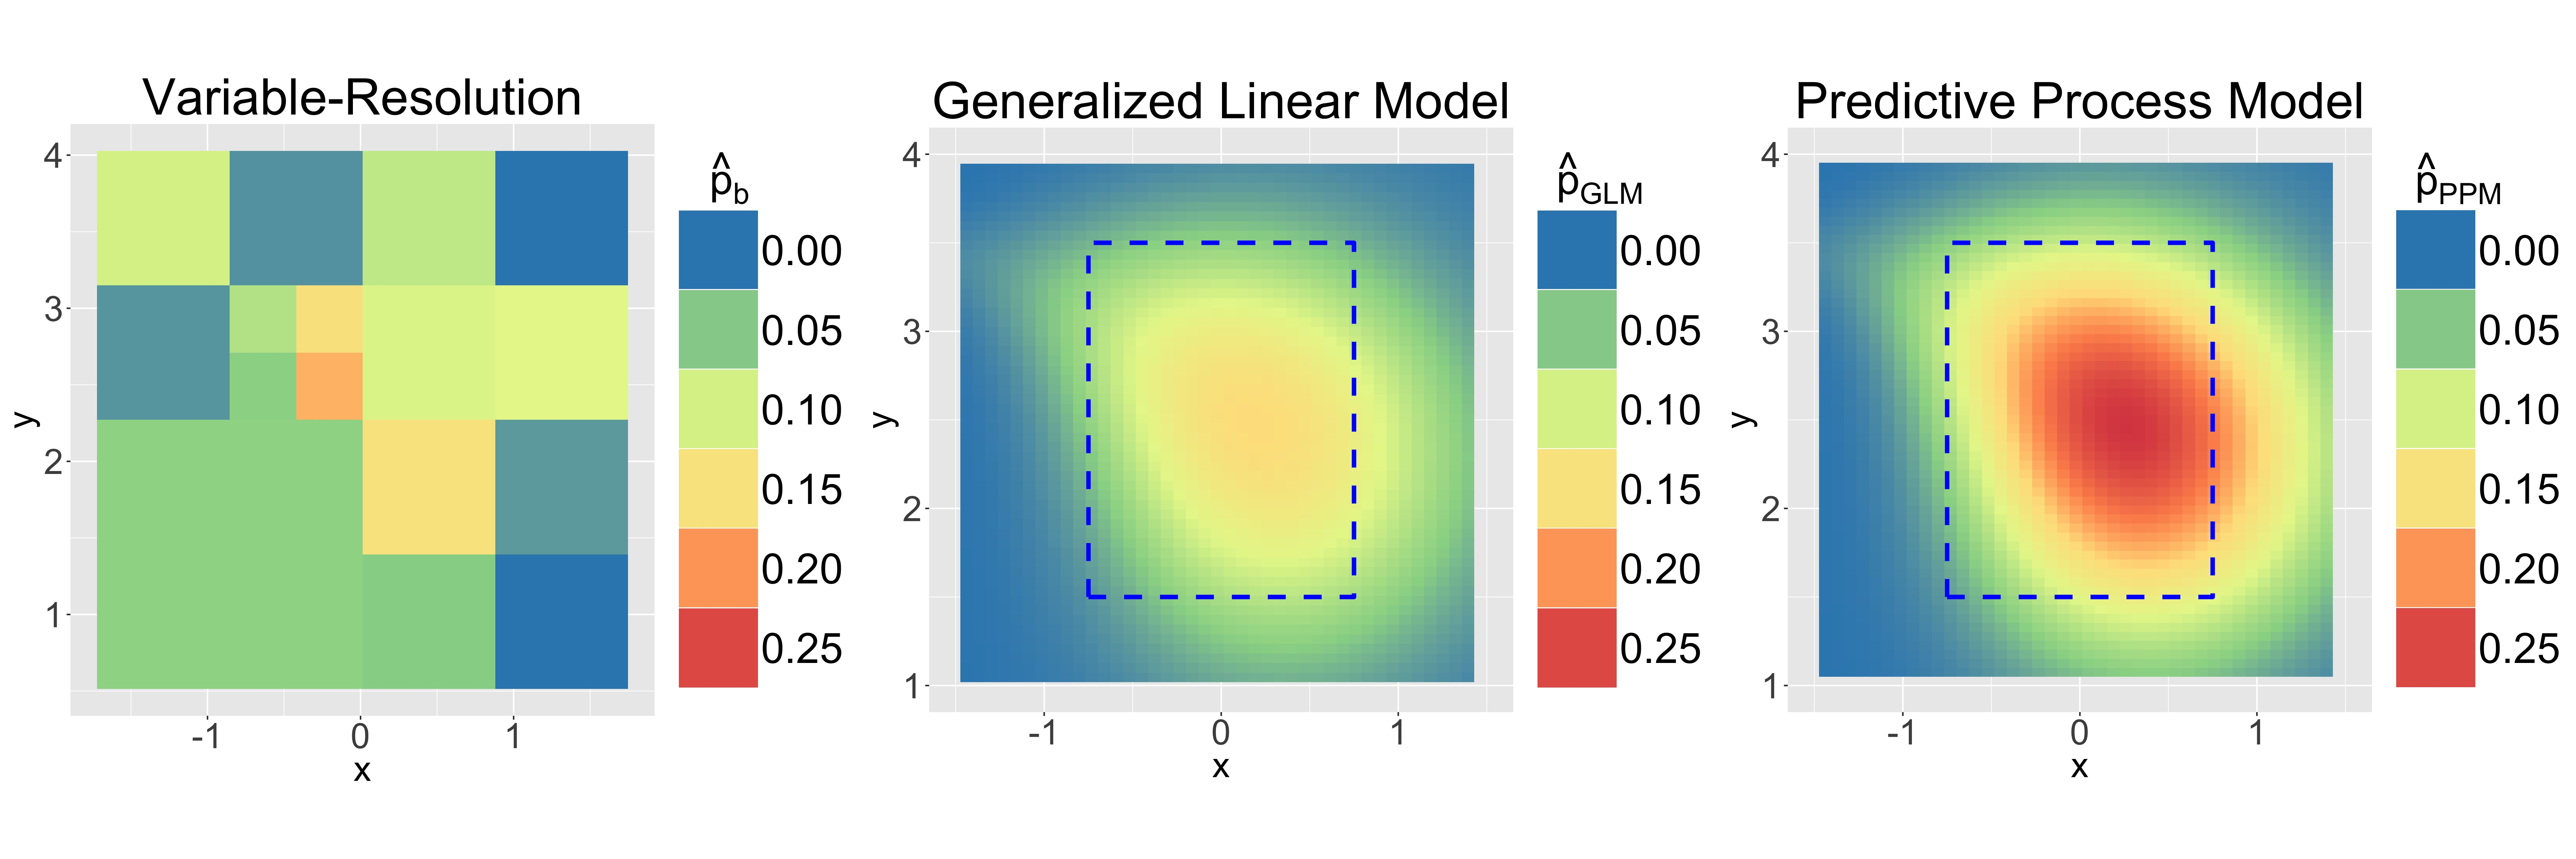
\includegraphics[scale=.05]{Images/VR_GLM_PPM.jpg}
	\caption{Empirical, generalized linear model, and predictive process model fits for a random subset of 1000 Jhonny Peralta observations. }
	\end{figure}

Changing the number of knots to 49, but still using n = 1000 observations, the fit generated 30,000 posterior draws in seven minutes. Finally, for n = 3000 observations, still with 49 knots, the fit generated 80,000 posterior draws in 54 minutes.

% 97 KNOTS ==================
% – Using 97 knots resulting from an nb < 200 cutoff, and n = 300 observations, spGLM(), about 3 mins. The trace plots did not suggest convergence.
% – Same, but n = 500, about 4 mins. does not look convergent. (10,000 itrtns)
% – n = 1000, 6.7 mins. Cnvrgnc *maybe* smidge better. time good!! (10,000 itrtns)
% – n=1000; 30,000 iterations; looks better. Not exactly convergent, but closer.
% 49 KNOTS ==================
% – 7 mins, n = 1000, knots = 49, 30K samples
% – X mins, n = 9172, knots = 49, “80,000 samples completed” but the dreaded rainbow pinwheel never went away when computer tried to resuscitate in morning. We’ll never know...
% – 54 mins, n = 3000, kn = 49, 80K samples

These results show tremendous promise in terms of speed. However, the sacrifice in dimensionality seems to have negatively impacted posterior convergence. Even with drastically more posterior draws, PPM trace plots showed less stability than Stan
fit posterior trace plots. Also, recall the Peralta data set contained 9,172 observations, and the final PPM fit described used only n = 3000 observations. Ideally we could fit a SPGLMM with all 9,172 observations to provide a point of comparison with the GLM fit; to answer the question---does a spatial random effect enhance the model sufficiently to justify its inclusion, given the increased computational demands? This question matters because in the long run we target a real-time evolving model, including more covariates and categories; recall the numerous aspects of the hitter vs. pitcher contest we omitted. With these goals in mind, next we explore a sophisticated approximation technique that promises to  reduce computation time further.

\section{Integrated Nested Laplace Approximations} \label{INLA} % =================
Integrated Nested Laplace Approximation (INLA), an approximation  based on advanced mathematical and computational techniques, works well for Bayesian hierarchical models with latent Gaussian {\bf Markov} random fields (GMRFs) \citep{Rue2007}. INLA works for GMRFs, but not for GRFs; INLA's speedy computations rely on sparse precision matrices. Therefore, in our setting, we must represent a GRF as a GMRF to use INLA; stochastic calculus supplies a link. A particular stochastic partial derivative of a Matern GRF equals a Gaussian random field white noise process. This identity provides a way to approximate a {\it Matern} GRF with a GMRF, in the form of a piecewise linear basis representation. The approach, known as Finite Element Method (FEM), essentially projects the SPDE onto a basis representation. The discrete representation consists of deterministic basis functions, defined by a triangulation of the domain, and GMRF weights. The basis representation, with a sparse precision matrix, qualifies for INLA. Scientists use FEM extensively in other fields.

\subsection{Gaussian Markov Random Fields}

In this section we formally define a GMRF, as in \citep{Rue2007}. Let $\pmb{x} = \{ x_{i}:i \in \mathscr{V} \}$, where $\mathscr{V} = \{1,\dots,n\}$, with $n = |\mathscr{V}|$-dimensional Gaussian random vector $\pmb{x}$. Now define graph $\mathscr{G} = \{ \mathscr{V}, \mathscr{E} \}$, containing vertices $\mathscr{V}$ and edges $\mathscr{E}$. Vertices $x_{i}$ and $x_{j}$ are conditionally independent given all other elements of $\pmb{x}$, if and only if $\{i, j\} \notin \mathscr{E}$. The neighborhood structure defined by this graph yields GMRF $\pmb{x}$ with respect to $\mathscr{G}$, where $i \sim j$ denotes $i$ neighbors $j$. The edges in $\mathscr{E}$ correspond exactly to the non-zero elements of the GMRF precision matrix $\pmb{Q}$; $\{ i, j \} \in \mathscr{E}$ if and only if $Q_{ij} \neq 0 \text{ for } i \neq j$. Non-zero elements of $Q_{ij}$ correspond to neighbors.


% To define a GMRF, first define multivariate Normal random vector $\pmb{w}(\pmb{s})$, for vector of locations $\pmb{s} \in \pmb{D} \subseteq \pmb{R}^{2}$. Define the GMRF mean as $\pmb{0}$. Now define a neighborhood structure whereby each random effect and its location, $w(\pmb{s}_{i})$, is a neighbor of $w(\pmb{s}_{j})$ according to a rule. It is required that $w(\pmb{s}_{i})$ is a neighbor of $w(\pmb{s}_{j})$ if an only if $w(\pmb{s}_{j})$ is a neighbor of $w(\pmb{s}_{i})$. This neighbor relationship is reflected in the covariance matrix of thte GMRF such that $\Sigma_{ij} \neq 0$ if an only if $w(\pmb{s}_{i})$ and $w(\pmb{s}_{j})$ are neighbors.

% $$ \pmb{w}(\pmb{s}) | \pmb{\theta} \sim MVN(\pmb{0}, \Sigma(\pmb{\theta})) $$

Integrated nested Laplace approximations (INLAs) require this GMRF structure. However, the model in this chapter contains a GRF. Therefore, we use stochastic partial differential equations (SPDEs), which provide an explicit link between GRFs and GMRFs. Section 1.5.2 describes the SPDE-based link. 

\subsection{Stochastic Partial Differential Equation (SPDE)} 

\cite{Whittle1954} declared Matern($\nu = 1$), not the exponential given by Matern($\nu = 1/2$), the ``elementary correlation'' function in two dimensions. The following defines the Matern family of covariance functions.
$$\text{C}(h) = \frac{\sigma^{2}}{2^{\nu - 1}\Gamma(\nu)}(\kappa h)^{\nu}K_{\nu}(\kappa h)$$
This parameterization includes range parameter $\kappa > 0$, smoothness parameter $\nu > 0$, scale parameter $\sigma^{2}$, and modified Bessel function $K_{\nu}(\cdot)$ \citep{Schabenberger2004}. Matern random fields solve the following SPDE \citep{Whittle1954}.
$$(\kappa^{2} - \Delta)^{\alpha/2}x(\pmb{s}) = \mathcal{W}(\pmb{s}),$$ 
This includes $\Delta = \sum_{i=1}^{d} \frac{\partial^{2}}{\partial x_{i}^{2}}$, the Laplace operator; spatial scale parameter $\kappa$, as in the Matern; smoothness parameter $\alpha$; and Gaussian spatial white noise process $\mathcal{W}(\pmb{s})$. The particular SPDE and Matern coupling dictates $\alpha = \nu + d/2$, where d = 2 for $\mathbb{R}^{2}$; and $$\sigma^{2} = \frac{\Gamma(\nu)}{\Gamma(\alpha)(4\pi)^{d/2}\kappa^{2\nu}}.$$
Based on \citep{Whittle1954}, \citep{Mondal2017}, and \citep{Lindgren2015}, we use $\nu = 1$, which implies $\alpha = 2$. This specification simplifies the SPDE to 
$$ (\kappa^{2} - \Delta)x(\pmb{s}) = \mathcal{W}(\pmb{s});$$ 
the Matern covariance to 
$$\text{C}(h) = \sigma^{2}(\kappa h)K_{1}(\kappa h);$$
and the variance to $\sigma^{2} = \frac{1}{4 \pi \kappa}$.

\subsubsection{Piecewise Linear Basis Representation}

The next step, known as the Finite Element Method, projects the SPDE onto a piecewise linear basis representation \citep{Simpson2012}. The basis representation,
$$ x(\pmb{s}) = \sum_{k=1}^{n} \psi_{k}(\pmb{s})x_{k},$$
contains deterministic basis functions, $\psi_{k}(\cdot)$; and weights $\pmb{x} = \{x_{1},\dots,x_{n}\}$, which constitute a GMRF. The two combine so that the distribution of $x(\pmb{s})$ approximates the Matern GRF that solves the SPDE, but retains a sparse precision matrix and its accordant computational advantages.

\subsubsection{Deterministic Basis Function}

A triangulation of the domain defines the deterministic component, $\psi_{k}(\pmb{s})$, of the basis representation. Figure 12 \citep{Simpson2012} illustrates how domain triangulation and determines a basis function.

  \begin{figure}[H]
	\centering 
	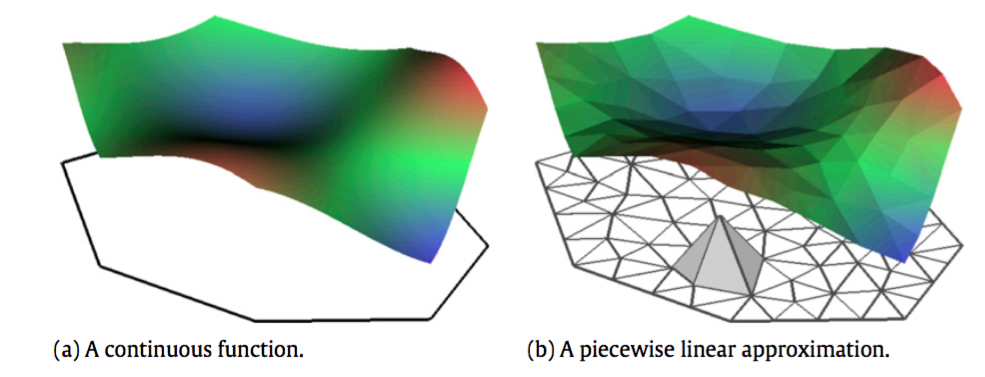
\includegraphics[scale=.4]{Images/PLBF.jpg}
	\caption{A Gaussian Markov random field, defined as the piecewise linear basis function $  x(\pmb{s}) = \sum_{k=1}^{n} \protect\psi_{k}(\pmb{s})x_{k}$, approximates a Matern GRF. This image illustrates how a triangular mesh over the domain determines basis functions $\protect\psi_{k}(\pmb{s})$ 
	\citep{Simpson2012}.}
	\end{figure}
	
Keep in mind that a realization of a GRF essentially constitutes a function, and Figure 12 shows how a discrete piecewise linear basis function approximates a continuous function \citep{Simpson2012}. Then, $\psi_{k}(\pmb{s}) = 1$ at the $k\text{th}$ vertex, $0$ at all other vertices, and surface function values for triangle interior points are linear combinations of the three home triangle vertices.

\subsubsection{GMRF Weights}

Stochastic calculus identities provide a way to calculate the weights in the basis representation. Define $\langle f, g \rangle = \int f(\pmb{u}) g(\pmb{u}) d\pmb{u}$, and find weights $\pmb{x}$ such that
$$ \left[ \left< \phi_{k}, (\kappa^{2} - \Delta)^{\alpha/2} \pmb{x} \right> \right]_{k = 1, \hdots, n} \overset{D}{=} \Big[ \langle \phi_{k}, \mathcal{W} \rangle \Big]_{k = 1, \hdots, n},$$
for a set of test functions $\phi_{k}$ \citep{Lindgren2011}. The appropriate weight vector $\pmb{x}$ gives the stochastic weak solution solution to the SPDE \citep{Mao2007}, \cite{Lindstrom2014}; we use the Galerkin solution, with $\alpha = 2$ and $\phi_{i} = \psi_{i}$ \citep{Lindgren2011}. Replace $\pmb{x}$ with basis function representation $\Sigma_{k}\psi_{k}w_{k}$,
$$ \left[ \left< \phi_{i}, (\kappa^{2} - \Delta)^{\alpha/2} \psi_{j} \right> \right]_{i,j}\pmb{w} \overset{D}{=} \Big[ \langle \phi_{k}, \mathcal{W} \rangle \Big]_{k}, $$
and let $\alpha = 2$ and $\phi_{i} = \psi_{i}$ as in the Galerkin solution:
$$ \Big(
\kappa^{2} [ \langle \psi_{i}, \psi_{j} \rangle ] + [ \langle \psi_{i}, -\Delta \psi_{j} \rangle ]
\Big) \pmb{w} \overset{D}{=} \Big[ \langle \psi_{k}, \mathcal{W} \rangle \Big]. $$
Let $\pmb{C}_{i,j} = \langle \psi_{i}, \psi_{j} \rangle$, and $ \pmb{G}_{i,j} = \langle \psi_{i}, - \Delta \psi_{j} \rangle$, so that
$$ \left(
\kappa^{2} \pmb{C} + \pmb{G} \right) \pmb{w} \overset{D}{=} N(\pmb{0},\pmb{C}).$$
For $\pmb{w} \sim N(\pmb{0}, \pmb{Q}^{-1})$, we have then
$$\pmb{Q}_{\kappa} = \left( \kappa^{2} \pmb{C} + \pmb{G} \right)^{T} \pmb{C}^{-1} \left( \kappa^{2} \pmb{C} + \pmb{G} \right).$$ 
However, $\pmb{C}_{ij}^{-1}$ has a sparse precision matrix, so replace $\pmb{C}$ with diagonal matrix $\widetilde{\pmb{C}}$,
$$ \widetilde{\pmb{C}}_{i,i} = \langle \psi_{i}, \pmb{1} \rangle = \int \psi_{i}(\pmb{s}) d\pmb{s}.$$ 
Note that this solution provides the distribution of the weights $x_{k}$, not $x(\pmb{s})$ itself, in the basis representation
$$ x(\pmb{s}) = \sum_{k=1}^{n} \psi_{k}(\pmb{s})x_{k}.$$
With this representation achieved, via the SPDE link, we move on to INLA.

\subsection{Integrated Nested Laplace Approximations (INLA)}

INLA consists of a series of calculations and approximations, to achieve estimates of key quantities. These quantities include the marginal posterior distributions for latent field parameters, $p(x_{i}|\pmb{y})$; and covariance hyperparameter posterior $p(\theta|\pmb{y})$. This means we never obtain posteriors $p(\pmb{x}|\pmb{y})$ and $p(\pmb{x},\pmb{\theta}|\pmb{y})$. We break the procedure into three steps to facilitate explanation, and details of them comprise the next three subsections.

\subsubsection{Step 1, Gaussian Approximation} % ======= ======

INLA begins by ``matching the mode and curvature at the mode'' of estimator $p_{G}(\pmb{x}|\pmb{\theta}, \pmb{y})$ to that of $p(\pmb{x}|\pmb{\theta}, \pmb{y})$ \citep{Rue2005}. INLA requires Gaussian priors for all parameters, excluding covariance hyperparameters. INLA also requires conditional independence, whereby $p(\pmb{y}|\pmb{x}, \pmb{\theta}) = \prod_{i} p(y_{i}|\pmb{x}_{i},\pmb{\theta})$. Our analysis satisfies this necessity, and therefore $$p(\pmb{x}|\pmb{\theta},\pmb{y}) \propto \text{exp}\left(-\frac{1}{2}\pmb{x}^{T}\pmb{Q x} + \sum_{i} \text{log }p(y_{i}|\pmb{x}_{i},\pmb{\theta}) \right).$$ With Gaussian priors and conditional independence satisfied, the INLA Gaussian approximation for $p(\pmb{x}|\pmb{\theta}, \pmb{y})$ takes the form
$$p_{G}(\pmb{x}|\pmb{\theta},\pmb{y}) \propto \text{exp} \left( -\frac{1}{2}(\pmb{x-\mu})^{T} (\pmb{Q} + \text{diag}(\pmb{c}) ) (\pmb{x - \mu}) \right),$$
where vectors $\pmb{c}$ and $\pmb{\mu}$ depend on second order Taylor expansions of $f(\pmb{x}) = \sum_{i} \text{log }p(y_{i}|\pmb{x}_{i},\pmb{\theta})$ about the mode \citep{Lindstrom2014}. A Newton-Raphson algorithm iteratively computes the mode and precision matrix until convergence \citep{Rue2009}. Step 2 uses this Gaussian approximation, $p_{G}(\pmb{x}|\pmb{\theta},\pmb{y})$, to approximate $p(\pmb{\theta}|\pmb{y})$.

\subsubsection{Step 2, Laplace Approximation}  % ====== ======

This step begins with two sides of a familiar identity, and its subsequent rearrangement.
\begin{align}
p(\pmb{y} , \pmb{x} | \pmb{\theta}) = p(\pmb{y} | \pmb{x}, \pmb{\theta}) p(\pmb{x} | \pmb{\theta})  &= p(\pmb{x} | \pmb{y}, \pmb{\theta}) p(\pmb{y} | \pmb{\theta}) \\
p(\pmb{y} | \pmb{x}, \pmb{\theta}) p(\pmb{x} | \pmb{\theta}) &= p(\pmb{x} | \pmb{y}, \pmb{\theta}) p(\pmb{y} | \pmb{\theta}) \\
\frac{p(\pmb{y} | \pmb{x}, \pmb{\theta}) p(\pmb{x} | \pmb{\theta})} {p(\pmb{x} | \pmb{y}, \pmb{\theta})} &= p(\pmb{y} | \pmb{\theta})  
\end{align}
We use this formulation of $p(\pmb{y} | \pmb{\theta})$ next, in the fundamental Bayesian proportionality.
\begin{align}
p(\theta|\pmb{y}) & \propto p(\pmb{y}|\pmb{\theta})p(\pmb{\theta}) \\
& \propto \frac{p(\pmb{y} | \pmb{x}, \pmb{\theta}) p(\pmb{x} | \pmb{\theta})}{p(\pmb{x} | \pmb{y}, \pmb{\theta})} \cdot p(\pmb{\theta})
\end{align}

For a given $\pmb{\theta}$, let $\pmb{x}_{0} = \text{argmax}_{x}p(\pmb{x}|\pmb{y},\pmb{\theta})$. Then,
$$ p(\pmb{\theta}|\pmb{y}) \approx \tilde{p}(\pmb{\theta}|\pmb{y}) \propto  \frac{p(\pmb{y} | \pmb{x}_{0}, \pmb{\theta}) p(\pmb{x}_{0} | \pmb{\theta})}{p_{G}(\pmb{x}_{0} | \pmb{y}, \pmb{\theta})} \cdot p(\pmb{\theta}),$$
where the Taylor approximation of $f(\pmb{x}) = \sum_{i} \text{log }p(y_{i}|x_{i})$, in $p_{G}(\pmb{x} | \pmb{y}, \pmb{\theta})$, expands about $\pmb{x}_{0}$. \cite{Tierney1986} showed this approximation matches Laplace approximation.  Then, we have approximate maximum likelihood estimate $\hat{\pmb{\theta}}_{\text{ML}} \approx \text{argmax}_{\theta} \tilde{p}(\pmb{\theta}|\pmb{y})$.

The results of Step 1 and Step 2 set the table for nesting and numerically integrating the Laplace approximations to obtain approximate marginal posteriors.

\subsubsection{Step 3, Numerical Integration} % === === === === ===
Numerical Integration over $\pmb{\theta}$, or elements of $\pmb{\theta}$, gives $p(x_{i}|\pmb{y})$ and $p(\theta_{i}|\pmb{y})$.
        $$ p(x_{j} | \pmb{y}) \approx \int p_{\text{G}}(x_{j}|\pmb{\theta, y})\tilde{p}(\pmb{\theta}|\pmb{y}) d\pmb{\theta} $$
        $$ p(\theta_{k} | \pmb{y}) \approx \int \tilde{p}(\pmb{\theta}|\pmb{y}) d\pmb{\theta}_{-k} $$

In summary, from a continuous domain the SPDE-INLA approximation procedure provides, with improved speed, posterior estimates for $p(\pmb{\theta}|\pmb{y})$, $p(\theta_{i}|\pmb{y})$, and $p(x_{i}|\pmb{y})$. The R package \verb|INLA| implements this procedure, with flexible SPDE arguments for domain triangulation.

\subsection{Bayesian Inference in R-INLA}